\documentclass{beamer} % default... %
%\documentclass[notes=only]{beamer} % notes only %
\usetheme{metropolis}

\usepackage{graphicx}
\usepackage{hyperref}
%\usepackage{listings}
\usepackage{minted}

\graphicspath{{figures/}}

%\usepackage{fontspec}
%\setsansfont{Ubuntu}
%\setmonofont{Ubuntu Mono}

%%%% some of my lkurusa-tools %%%%

\newcommand*{\emailify}[1]{$<$#1$>$}
\newcommand*{\myemail}{\emailify{levex@linux.com}}
\newcommand*{\ptrace}{\texttt{ptrace}}
\newcommand*{\ptraceman}{\texttt{ptrace(2)}}
\newcommand*{\sig}[1]{\texttt{SIG#1}}
\newcommand*{\sigsegv}[0]{\sig{SEGV}}
\newcommand*{\sigtrap}[0]{\sig{TRAP}}
\newcommand*{\sigill}[0]{\sig{ILL}}

%%%%%%%%

\title{Let's write a Debugger!}
\author{Levente Kurusa \myemail}
\date{Imperial College London}
\institute{\texttt{linux.conf.au 2018}, Sydney, Australia \hfill January 25, 2018}

\begin{document}
\maketitle

\begin{frame}{Who am I?}
\begin{itemize}
  \item Final year undergraduate at Imperial College London
  \item Previously at Apple and Red Hat
  \item Now researching different ways of operating system construction
  \item Low-level hacker
\end{itemize}
\end{frame}

\section{History of debuggers}

\begin{frame}{Single user machines}

\begin{columns}
\column{0.5\textwidth}
\begin{itemize}
    \item One of the first computers in the world
    \item Small application was loaded at the top of the memory
      \begin{itemize}
          \item single step
          \item examine registers
          \item read/write memory
      \end{itemize}
\end{itemize}

\column{0.5\textwidth}
\metroset{block=fill}
\begin{block}{TX-0 at MIT}
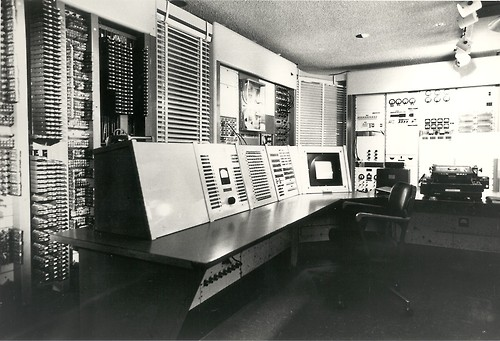
\includegraphics[width=0.4\paperwidth]{tx0.jpg}
\end{block}

\end{columns}

\note{
    Prepunched cards with the code\\
    Names like DDT and ODT
}

\end{frame}

\begin{frame}{Batch processing machines}
\includegraphics<1>[width=\textwidth]{punch_card_stack.jpg}
%TODO: https://en.wikipedia.org/wiki/Punched_card#/media/File:Punched_card_program_deck.agr.jpg
%TODO: Mention license at the end and attribute
\pause
Debugged by putting macro call in the punch card and generating:
\begin{itemize}
    \item Snapshots \textit{(register dump)}
    \item Core dumps \textit{(contents of memory)}
\end{itemize}

\note{
    A different class of machines was also on the rise. \\
    Submit a stack of punch cards and wait for the result at the end of the day
}

\end{frame}

\begin{frame}[fragile]
\frametitle{printf}

Then came CTSS \textit{(Compatible Time-Sharing System)}, one of the first time-sharing operating
systems! \par
\vspace{.5cm}
Debugging suddenly became interactive.

\metroset{block=fill}
\begin{block}{printf-debugging}
\begin{minted}{c}
  *ptr = 1337;
  printf("Did we crash at line %d?\n", __LINE__);
  *((int *) 0) = 1337;
  printf("Did we crash at line %d?\n", __LINE__);
\end{minted}
\end{block}

\end{frame}

\begin{frame}{Unix-es}
\begin{itemize}
    \item The first version of Unix had a debugger called, \texttt{DB}
    \item GNU had \texttt{GDB} and \texttt{LLDB}
    \item For Plan 9, \texttt{ADB} was created
\end{itemize}
\vskip.5cm
These debuggers should be familiar!
\end{frame}

\section{Tracing processes}

\begin{frame}[fragile]
\frametitle{ptrace}

Most debuggers heavily rely on a system call known as \ptrace.
\vskip1cm
\metroset{block=fill}
\begin{block}{The prototype of \ptraceman}
\begin{minted}{c}
#include <sys/ptrace.h>

long ptrace(enum __ptrace_request request, pid_t pid,
                   void *addr, void *data);
\end{minted}
\end{block}
\end{frame}

\begin{frame}{Signals}
\begin{center}
    \only<1->How does \mintinline{c}{int a = 3, b = 0, c = a / b} result in a \sig{FPE}?
\end{center}
\only<2->{\begin{enumerate}
    \item<2-> Division by zero is noticed by the CPU
    \item<3-> The CPU raises a Divide-by-zero exception \texttt{(\#DE)}
    \item<4-> A handler in the kernel is eventually called
    \item<5-> The kernel sends a \sig{FPE} to the offending process
    \item<6-> Your signal handler is called (or not if it is \sig{KILL})
\end{enumerate}
}
\end{frame}

\begin{frame}{Implementation}
\begin{itemize}[<+- | alert@+>]
    \only<1->{
        \item<1-> \alert<2,3>{Enable tracing}
            \only<3->{
                \begin{itemize}
                    \item \texttt{PTRACE\_TRACEME}
               \end{itemize}
            }
        \item<1-> \alert<4,5>{Run until system call}
            \only<5->{
                \begin{itemize}
                    \item \texttt{PTRACE\_SYSCALL}
                    \item \texttt{PTRACE\_SYSEMU}
                \end{itemize}
            }
        \item<1-> \alert<6,7>{Monitoring registers}
            \only<7->{
                \begin{itemize}
                    \item \texttt{PTRACE\_PEEKUSER / PTRACE\_POKEUSER}
                    \item \texttt{PTRACE\_GETREGS / PTRACE\_SETREGS}
                \end{itemize}
            }
        \item<1-> \alert<8,9>{Single stepping}
            \only<9->{
                \begin{itemize}
                    \item \texttt{PTRACE\_SINGLESTEP}
                \end{itemize}
            }
    }
\end{itemize}
\end{frame}

\section{Architectural support}

\begin{frame}{Interrupting a process}

\only<1->{
\begin{center}
    {\Large \texttt{PTRACE\_SINGLESTEP}}
\end{center}
}

\only<2->{
    \begin{itemize}
        \item<2-> \mintinline{asm}{ud2} \hfill (machine code: \mintinline{c}{0x0F 0x0B})
                \begin{itemize}
                    \item Triggers \texttt{\#UD}
                \end{itemize}
        \item<3-> \mintinline{asm}{int $3} %$% <-- to fix tex studio highlighting lol
                \hfill (machine code: \mintinline{c}{0xCC})
                \begin{itemize}
                    \item Triggers \texttt{\#BP}
                \end{itemize}
    \end{itemize}
}

\end{frame}

\begin{frame}{Debug registers}
\begin{itemize}
    \item<1-> \texttt{DR0-DR3}: Linear addresses
    \item<2-> \texttt{DR4} \& \texttt{DR5}: Obsolete aliases to \texttt{DR6} \& \texttt{DR7}
    \item<3-> \texttt{DR6}: Debug control\\
        Contains bitmasks for:
        \begin{itemize}
            \item 1, 2, 4 or 8 bytes monitored
            \item Break on read, write, execute, or read+write
        \end{itemize}
    \item<4-> \texttt{DR7}: Debug status \\
        Bitmask showing which of \texttt{DR0-DR3} triggered the \texttt{\#DB}
\end{itemize}
\end{frame}

\begin{frame}{Thanks!}
\begin{center}
Thank you for your attention! \par
\end{center}

Twitter: @iLevex \hfill Email: \myemail \\
GitHub: levex \hfill Website: \url{http://osdev.me/}

\vspace{1cm}

\begin{small}
The \LaTeX\hskip1mm theme is available at \url{github.com/matze/mtheme}

Both the theme and the talk are licensed under the
\href{http://creativecommons.org/licenses/by-sa/4.0/}{CC-BY-SA 4.0 International license}.

\end{small}

\end{frame}

\end{document}
